\documentclass[a4paper,11pt]{article}
\usepackage[utf8]{inputenc}
\usepackage{algorithmic}
\usepackage{algorithm}
\usepackage{pst-plot}
\usepackage{graphicx}
\usepackage{endnotes}
\usepackage{graphics}
\usepackage{floatflt}
\usepackage{wrapfig}
\usepackage{amsfonts}
\usepackage{amsmath}
\usepackage{verbatim}
\usepackage{hyperref}
\usepackage{multirow}
\usepackage{pdflscape}
\usepackage{enumitem}
\usepackage[normalem]{ulem}

\usepackage{hyperref}
\hypersetup{pdfborder={0 0 0 0}}

\pdfpagewidth 210mm
\pdfpageheight 297mm 
\setlength\topmargin{0mm}
\setlength\headheight{0mm}
\setlength\headsep{0mm}
\setlength\textheight{250mm}	
\setlength\textwidth{159.2mm}
\setlength\oddsidemargin{0mm}
\setlength\evensidemargin{0mm}
\setlength\parindent{7mm}
\setlength\parskip{0mm}

\newenvironment{exercise}[1]{\paragraph{#1}\ \\}{
\medskip}
\newcommand{\question}[2]{\setlength\parindent{0mm}\ \\$\mathbf{Q_#1:}$ #2\ \\}

\author{\large{Tambet Matiisen, Raul Vicente, Zurab Bzhalava}}
\title{\huge{3rd Baltic-Nordic Summer School on Neuroinformatics (BNNI 2015)}\\\LARGE{Practice on Artificial Neural Networks}}

\begin{document}
\maketitle

%
% Intro
%
The 2014 Nobel prize in Physiology was awarded to Dr. John M. O'Keefe, Dr. May-Britt Moser and Dr. Edvard I. Moser for discovering particular cells in the brain that provide the sense of place and navigation. In this practice session, we are going to use computational approach to study the animal "GPS" system. In particular, we are going to use artificial neural networks to predict a rat's position based just on its hippocampal neural activity.

At first we divide the experimental arena into 16 blocks and approach this as a classification problem. Next we make the task harder by trying to predict rat's position (X and Y coordinates) directly, i.e. approach this as a regression problem. Finally we look if we can automate the tedious task of hyperparameter optimization using Whetlab. 

The data we use is multi-neuron electrophysiological recordings from the Buzsaki lab in New York. The data has been preprocessed as number of spikes in 200ms time window.

%
% ANN
%
\section{Artificial Neural Networks}

Tuning artificial neural networks can be frustrating experience. Many people have tried and given up before they start to get any useful results. In this practice session we hope to give you step-by-step guidelines, how to tune the learning parameters of neural network and squeeze out  maximum performance from them. But before that we need to have the basic understanding how artificial neural networks work.

Artificial neural network consists of interconnected nodes, sometimes called "neurons". Some of those nodes are input nodes - they receive information from the outside world. Some of them are output nodes - they provide the results of calculation. Finally there are hidden nodes, which are just intermediate steps of computation.

\begin{figure}[h]
	\centering
	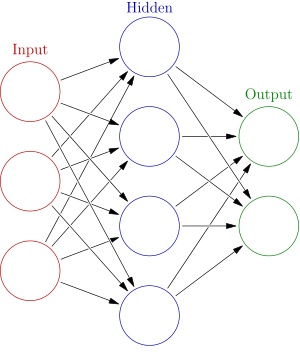
\includegraphics[width=0.25\textwidth]{ann.png}
	\caption{Artificial neural network with one hidden layer.}
\end{figure}

Nodes of artificial neural network are organized into layers. There are no connections between nodes in the same layer, only between layers - input layer nodes are connected to first hidden layer nodes, first hidden layer nodes are connected to the second hidden layer nodes and so on until last hidden layer is connected to the output layer. In simplest feed-forward neural networks, the connections are in one direction only - from input towards output.

\begin{figure}[h]
	\centering
	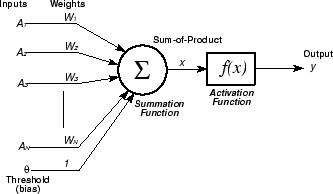
\includegraphics[width=0.55\textwidth]{neuron.png}
	\caption{Artificial neuron.}
\end{figure}

While artificial neurons are inspired by their biological counterparts, they are just cartoonish simplifications of actual neurons. Typical artificial neuron just multiplies its inputs with respective weights, sums the results and applies activation function. Common activation functions used are $sigmoid$ (squashes any real value between $0$ and $1$), $tanh$ (squashes any real value between $-1$ and $1$) and $ReLU$ (rectified linear unit, just takes $max(x, 0)$). The purpose of activation function is to add non-linearity into calculations.

\begin{figure}[h]
	\centering
	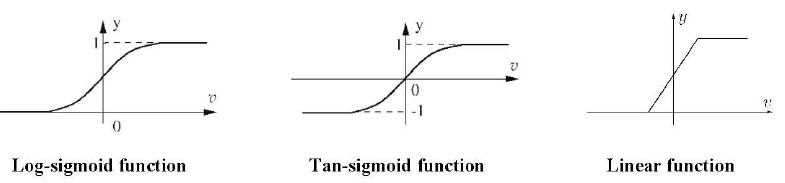
\includegraphics[width=0.8\textwidth]{activation_functions.png}
	\caption{Common activation functions.}
\end{figure}

The beauty of artificial neural networks is, that they can learn to map inputs to outputs, given enough examples. The learning is accomplished by changing weights between neurons. There is theoretical result, that any function can be approximated to given precision using artificial neural network with one hidden layer. In practice this result is irrelevant, because the claim that function can be represented by network doesn't say anything if the function can be learned by the network. Still the thing to remember from this is, that artificial neural networks are nothing more, than universal function approximators.

How the learning works in artificial neural networks? It all starts with loss function, which measures how good networks' prediction is, how well its outputs match the expected values. Small loss is good, big loss is bad. The most common loss function is mean squared error (MSE) - you just square all differences between predicted and expected values, sum over all output nodes and take mean over training batch. If ouputs of your network are probabilities, then you would use different loss function (cross-entropy loss), but the general idea stays the same.

Now, to learn you need to change the weights in a way, that loss function decreases. How do you do that? The most common method is gradient descent - you take partial derivative of the loss function with respect to each weight and this gives you estimate, how much you need to change this particular weight to make loss function go down. Gradient is nothing more, than vector of loss function partial derivatives with respect to each weight. To calculate those derivatives efficiently in artificial neural network there is algorithm called backpropagation. Basically it applies chain rule to produce derivatives of bottom layers from derivatives of upper layers. We are not going to dwelve into details here, just assume that somehow you know the gradient, how much you should add to or subtract from each weight to make the loss decrease.

\begin{figure}[h]
	\centering
	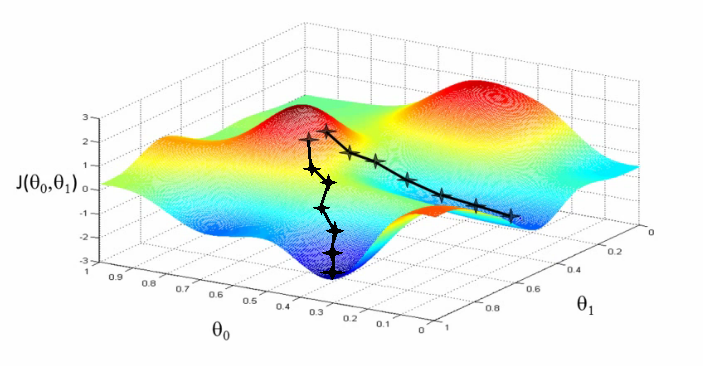
\includegraphics[width=0.8\textwidth]{gradient_descent.png}
	\caption{Gradient descent.}
%
% $J(\theta_1,\theta_2)$ is the loss function, $\theta_1$ and $\theta_2$ are the weights (suppose we have only two of them).
%
\end{figure}

Complex nature of artificial neural network means, that there is no one set of weight values, for which loss function has minimal value, i.e. it is non-convex optimization problem. Often the metaphore "loss landscape" is used - if you would plot loss value over many weight value combinations, then this would form landscape of many hills and valleys. If you just follow the gradient (steepest descent), then it is easy to get stuck in local minima (shallow valley). People have come up many techniques to work around this issue, but in principle it remains unresolved. Good news is, that many local minimas are pretty good and there are plenty of them.

%
% Classification
%
\section{Classification}

In this exercise we divide the arena into 16 regions and try to predict the region where the rat is from activity of 61 neurons in hippocampal area of the brain.\\

Run the code in \texttt{classification.m} and observe the results:

\begin{enumerate}
	\item First you should see baseline performance of linear classifier. This is there to just remind you, that artificial networks are heavy artillery and should be used only if simpler methods don't give satisfactory results. 
	\item Then you should see training progress of artificial neural network. You can ignore the command-line output and concentrate on the two figures shown during training:
	\begin{itemize}
		\item The first one shows loss function value for both training and validation set. In this case we use cross-entropy loss function. Its value is actually meaningless, we are more interested in the dynamics - does it decrease, how fast, is it stable?
		\item The second figure shows misclassification rate - the fraction of training samples, for which the predicted class was wrong. You can get accuracy by subtracting this number from 1. Again, both training and validation set error rates are shown.
	\end{itemize}
	Usually those two graphs are correlated, so it suffices to only pay attention to the latter. Also you care more about the validation set performance, than training set performance.
	\item After that you should see accuracy of neural network printed out. At first it might not be much better than linear classifier.
	\item Finally confusion matrix is shown. Confusion matrix shows common errors - which classes were mistaken for other classes.
\end{enumerate}

\textbf{Your job is to tune this neural network to have accuracy at least 70\%.}

\begin{figure}[h]
	\centering
	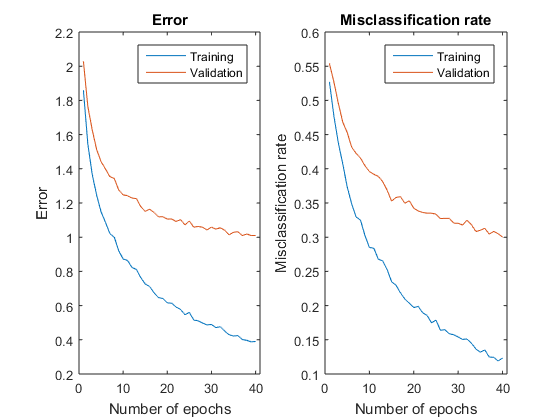
\includegraphics[width=0.9\textwidth]{training_loss.png}
	\caption{Example of network achieving 70\% accuracy.}
\end{figure}

How do you go about that? 

\begin{enumerate}
	\item First you should start by finding optimal learning rate. Learning rate is the one most important learning parameter, it determines the step size on loss landscape. 
	\begin{itemize}	
		\item Too big learning rate - you step over valleys and never into them. 
		\item Too small learning rate - you end up in closest valley, that might not be the deepest. 
	\end{itemize}
	Usually you try learning rate in decreasing powers of 10, i.e. 1, 0.1, 0.01, 0.001 and so on. Repeat  until graphs are stable and validation accuracy doesn't improve any more. Basically you want to use the highest learning rate, that does not blow up your loss.
	\item Then you might want to increase the number of hidden nodes to see if validation accuracy improves. More hidden nodes means the more complicated functions the network can express. Usually you do it in powers of 2, i.e. use twice as much hidden nodes as previously.
	\item After that you should use momentum to speed up learning. Momentum adds inertia to weight updates - each update also includes some fraction of previous weight update, forcing faster movement on long descends in one direction. Sometimes momentum may overshoot resulting in zig-zags on graphs, but usually it helps to reach to minima faster. Usual values to try are 0.5, 0.9 and 0.95.
	\item By now you should observe massive overfitting - training set error is much smaller than validation set error. Basically network memorizes the training set and doesn't generalize to the validation set. There are several ways how to deal with overfitting:
	\begin{description}
		\item[Get more training data.] Data is the most effective regularizer, so if possible you should always use that option. The reality is, that often it is not easy to get additional data, and then the following methods come to play.
		\item[Use weight decay.] This is well-known technique, that forces weights to have small values. It is implemented by adding regularization term to loss function, which results in weights decreased by some fraction of previous weight value during each training iteration (hence "weight decay"). You should start with low values of $10^{-4}$ and go up in powers on 10 until validation set accuracy doesn't improve any more.
		\item[Use dropout.] Dropout disables some subset of hidden nodes during training. This forces nodes to be more individualistic, because they are not able to rely on others. During testing hidden node values are multiplied by the same fraction to produce on average the same amount of input to next layer nodes. This functions also as a crude approximation to ensemble method - basically we are averaging results of many networks with shared weights. Common dropout fraction to use is 0.5, but in some cases lower values might work as well.

\begin{figure}[h]
	\centering
	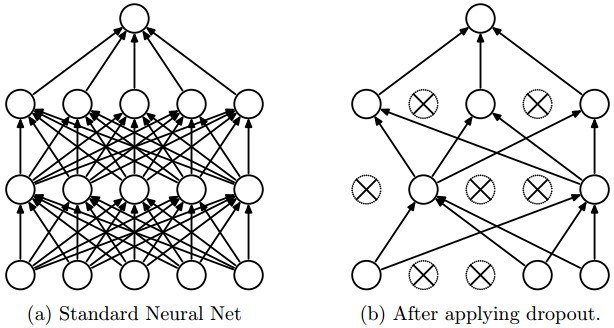
\includegraphics[width=0.6\textwidth]{dropout.jpg}
	\caption{Dropout.}
\end{figure}

	\end{description}

	Finally, some amount of overfitting is inevitable and healthy with neural networks. So as long as validation set accuracy improves, don't worry too much about it.

	\item Once you think your learning parameters are good enough, you should try to learn longer - increase the number of epochs. One epoch is full training session over entire training set. Usually loss function plateaus at some point and there is no point training any further. You should figure out where this point is by trying say 100 epochs. Then for further finetuning you can use the number of epochs before plateau is reached.

	\item As gradient descent explores the loss landscape, there might be gradually more fine-grained valleys to descend to. With initial learning rate you may just step over those valleys or step out of them. For that reason it is usually good idea to try smaller learning rate just before loss function has plateaued. Usually you do it in powers of 10, i.e. multiply learning rate by 0.1. But DeepLearnToolbox applies scaling rate after each epoch, so you need to calculate approximate per-epoch scaling rate, that results in 0.1 multiplier after $n$ epochs. This can be calculated by

$$
scaling\_learningRate = \sqrt[n]{0.1}
$$

\end{enumerate}

Things you shouldn't invest too much effort into:

\begin{itemize}
	\item Batch size. In stochastic gradient descent (SGD) you divide training set into batches of random samples and train one batch at a time. You use average gradient of all samples in batch to perform the weight update. If batch size is too small, your gradient may not point towards minima for entire training set and gradient descent will walk around randomly. If batch size is too big, then each training iteration is just very time consuming. Use smallest batch size, that is sufficiently representative of training set distribution. Often this is more restricted by the amount of memory your GPU has or how many parallel computations it can handle.
	\item Activation function. For small shallow networks use $tanh$. Modern deep networks use $ReLU$ to combat the vanishing gradient problem and maximize performance. But this is not so much issue with small networks.
	\item Depth of the network. While hierarchical representation of features is the main selling point of artificial neural networks, the benefits of hierarchy show up only with more complex networks architectures like convolutional networks. These networks make use of the locality property of information. For small fully-connected networks usually one-two layers is enough.
 \end{itemize}

%
% Regression
%
\section{Regression}

In this exercise we try to predict rat's location directly. This time we are going to use activity of all 70 neurons as input. Outputs of the network are the X and Y coordinates of the rat.\\

Run the code in \texttt{regression.m} and observe the results:

\begin{enumerate}
	\item First you should see baseline performance of linear regression. The result is given as an average Euclidian distance between predicted and actual rat location.
	\item Then you should see training progress of artificial neural network. This time there is only one figure - the loss. For regression we are using the standard mean square error loss (MSE). Again you should pay more attention to validation set loss than training set loss.
	\item After that you should see the performance of neural network printed out. Again, at first it might not be much better than linear regression.
	\item Finally 100 examples of predicted and actual locations are shown. You can tune the number of examples shown or duration of pause between them.
\end{enumerate}

\textbf{Your job is to achieve as good average distance as you can!}\\

Use all the tricks you learned from previous exercise. As dataset is bigger this time, you might initially want to choose smaller subset of samples to work with. This way training completes in minutes and you can iterate fast. Once you have successfully overfitted the smaller dataset, try full dataset and see if performance on validation set improves.

\end{document}
